\documentclass[conference]{IEEEtran}
\IEEEoverridecommandlockouts
% The preceding line is only needed to identify funding in the first footnote. If that is unneeded, please comment it out.
\usepackage{cite}
\usepackage{amsmath,amssymb,amsfonts}
\usepackage{algorithmic}
\usepackage{graphicx}
\usepackage{textcomp}
\usepackage{xcolor}
\usepackage{array}
\usepackage[section]{placeins}
\usepackage{float}
\usepackage{listings}


\def\BibTeX{{\rm B\kern-.05em{\sc i\kern-.025em b}\kern-.08em
    T\kern-.1667em\lower.7ex\hbox{E}\kern-.125emX}}
\begin{document}

\begin{titlepage}
	\title{Cheap Autonomous Rovers for Multi-Agent Applications\\
		{\footnotesize \textsuperscript{*}Freedom Rover Units}
		\thanks{}}

	\author{\IEEEauthorblockN{1\textsuperscript{st} Jordy A. Larrea Rodriguez}
		\IEEEauthorblockA{\textit{Department of Electrical and Computer Engineering} \\
			\textit{University of Utah}\\
			Salt Lake City, USA \\
			Jordy.larrearodriguez@gmail.com}
		\and
		\IEEEauthorblockN{2\textsuperscript{nd}  Brittney L. Morales}
		\IEEEauthorblockA{\textit{Department of Electrical and Computer Engineering} \\
			\textit{University of Utah}\\
			Salt Lake City, USA \\
			brittneymrls@gmail.com}
		\and
		\IEEEauthorblockN{3\textsuperscript{rd} Misael Nava}
		\IEEEauthorblockA{\centerline{Department of Electrical and Computer Engineering} \\
			\textit{University of Utah}\\
			Salt Lake City, USA \\
			misaelnava812@gmail.com}
	}
	\maketitle
\end{titlepage}

\twocolumn

\begin{abstract}
The state of the art in autonomous swarms employs a decentralized model consisting of multi-agent networks. These robotic collaborative systems hold the potential to adapt to new environments and optimize individual performance to specific tasks without having to deal with global systems prone to single points of failure. Our team's focus lies therein in developing a multi-agent system capable of a decentralized network. The swarm will incorporates three two-wheel differential drive rovers interfaced through the Robot Operating System (ROS) via wifi telecommunication through the micro-ROS agent service. The central bay system consists of a single laptop to communicate objectives for the agents to complete (carefully designed demos). Our development stack will leverage ROS for project management, simulation capabilities, navigation libraries, and native server-client model in robotics applications. The rovers AI will incorporate simultaneous localization and mapping (SLAM) techniques for RT positioning based on a priori grid or map; thus, facilitating navigation through improved state space mapping. Thus, we introduce FRU-bot, an autonomous platform capable of deployment in decentralized and centralized systems.
\end{abstract}

\begin{IEEEkeywords}
Decentralized Communication, Swarm Communication, Multi-agent, ROS, Gazebo
\end{IEEEkeywords}

\section{Introduction}
\begin{figure}
	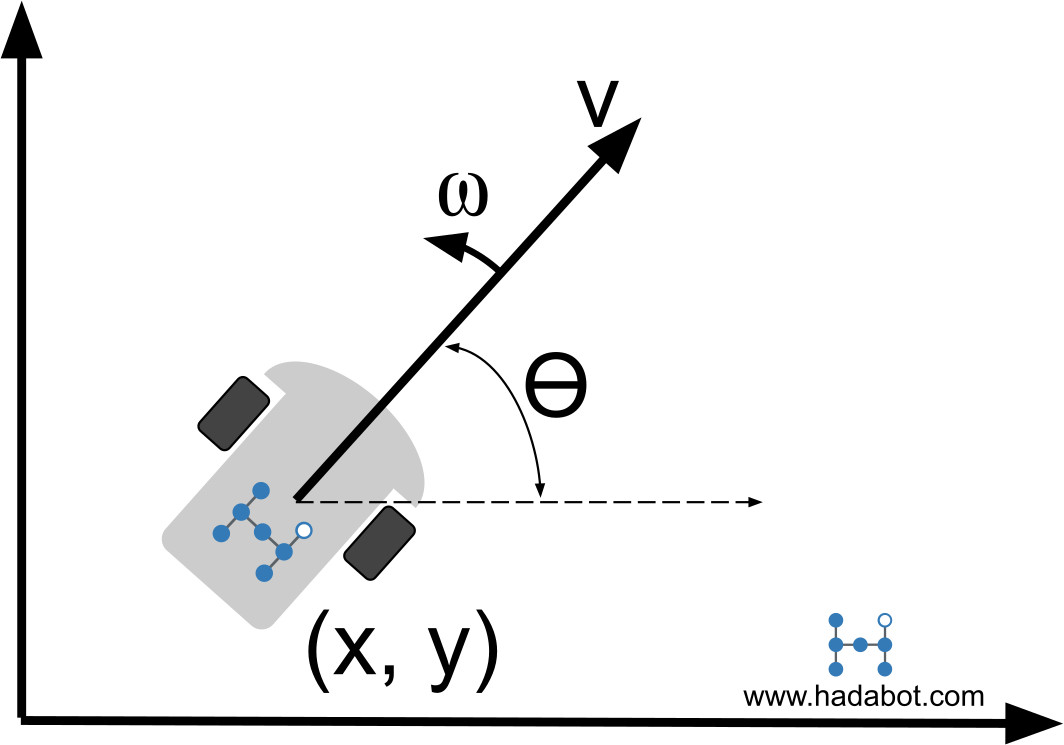
\includegraphics[width=\linewidth]{hadabot_unicycle_diagram_01.jpg}
	\caption{Graphical representation of 2D robot pose information standard to 2 wheel robots \cite{RN109}.}
\end{figure}
Our team's primary objective was to design a networked swarm of rovers capable of collaborative mapping, obstacle avoidance, and cooperative task execution. Our aim is to establish a foundational system that aids in Search and Rescue operations and facilitates research in multi-swarm rover technology. Presently, we've achieved success in creating rovers equipped with mapping capabilities, allowing real-time simultaneous visualization of surrounding areas within a simulation Moreover, our accomplishment includes developing these rovers at an affordable price point, under \$100 each. This cost-efficient solution stands in contrast to market offerings that typically start at \$300 for a turtle bot with a Jetson nano and increase steeply thereafter.

\section{Background} 
A plethora of elements must come together to successfully deploy a swarm of decentralized agents. Our system requires a working knowledge in both the physical and abstract. The agents are subject to their physical characteristics: i.e., their circuitry, power consumption, mechanical components, sensors, processing power, and geometry to navigate and respond to an environment. The complexity that drives cyber-physical systems is what largely makes robotics difficult. An agent must be able to function perfectly in a world with a continuous state space. Today, researchers are seeing a high degree of success with robots that incorporate mathematical and data driven modeling that leverages the superior computational capabilities of modern processors to solve complex continuous problems in robotics. 
\subsection{Common Robot Autonomous Platforms} Common mobile platforms for autonomous robots encompass a range of designs tailored to diverse applications within the field of robotics. Wheeled platforms, such as differential drive and omnidirectional robots, are popular choices due to their simplicity and efficiency in navigating various environments. Differential drive platforms use two powered wheels, allowing the robot to turn and move forward or backward by adjusting the speeds of the wheels. Omnidirectional platforms, on the other hand, utilize special wheel configurations to achieve unrestricted movement in any direction. Lastly, tracked platforms offer enhanced traction and stability, making them suitable for challenging terrains.

One notable platform is the TurtleBot 3, a popular open-source robot platform widely used for research and education. TurtleBot 3, developed by ROBOTIS, is a compact and modular robot equipped with various sensors, including a 360-degree lidar sensor, a camera, and inertial measurement units (IMUs). Its differential drive system allows for omnidirectional movement, making it versatile for navigation in dynamic environments. The TurtleBot 3 is often employed in the development and testing of autonomous navigation algorithms, mapping techniques, and obstacle avoidance strategies. Its affordability, ease of use, and vibrant community support make it an attractive choice for researchers, students, and hobbyists interested in exploring the intricacies of autonomous robotics.

\subsection{Robot Localization}
\begin{figure}
	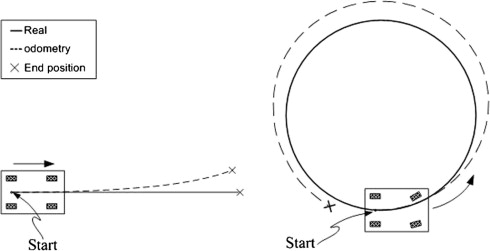
\includegraphics[width=\linewidth]{odometry_error.jpg}
	\caption{Graphical representation of basic odometry error as a robot follows a reference trajectory \cite{RN206}.}
\end{figure}
Normally, robots use a wide range of sensors to inform themselves about the surrounding environment. Our agents, for example, rely on a 6 axis inertial measurement unit (IMU) and rotatory encoders to produce an \{$X$, $Y$, $\theta$, $\dot{X}$, $\dot{Y}$, $\dot{\theta}$, $\ddot{X}$, $\ddot{Y}$\} state configuration at every time step by considering physical properties and mechanics (Fig. 1). However, a frequent problem with using rudimentary techniques solely for odometry is that error propagated at each time step due to environmental conditions, sensor specifications, electrical noise, and rounding error can deviate a naive agent during localization. The problem persists even with the use of a known map and highly accurate sensors. Consider how a human might traverse a city by using a map. The human could ensure their own position by simply pondering their place in respect to features of the map like buildings, intersections, or street signs. Even if the human absent mindlessly navigated the city, they could triangulate their location by simply calculating their positions based on observations (such as the coffee shop across the street). Our robots, incorporate a Kalman ExFor an agent, SLAM leverages known knowledge of poses at past time steps and emissions or observations (sensor readings) made as the agent accumulates error through basic odometry to calculate probabilities of where the agent can be in space. Any number of sensors that detect 'emissions' from the environment can be used for SLAM; however, 2D lidar and cameras are regularly used for the high degree of precision awarded. Agents are capable of both learning a new environment and updating a known map with SLAM; thus, justifying our deployment of SLAM to improve the navigation capabilities of each agent.

\subsection{Robot Kinematics} <Jordy>

\subsection{ROS2 and Open Source Frameworks} <Jordy>

\subsection{Robot Description and Transformation Trees} <Jordy>

\subsection{Gazebo for Robot Simulation} <Jordy>

\subsection{Autonomous Navigation} <Jordy>

\subsection{Multi-Agent Swarm Systems} <Jordy>

\section{Project Implementation}
\subsection{Preliminary Robot Chassis}

Our rover is designed with two distinct levels, both 3D-printed boards with holes to screw in different components. The upper level features the LiDAR for a clear view, with the wires going through the center of the 3D-printed board.
On the lower level, our lithium batteries are securely attached using Velcro at the rear. The power board is positioned at the front, fastened by two of the four poles securing both levels.
Beneath the bottom board,  two TT motors are firmly fixed to the 3D-printed board using screws, alongside encoders secured with a hot glue gun adjacent to the motors. Wires from the encoders, motors, and LiDAR are routed towards the rear, adjacent to the batteries, and connected to our power board. This central hub houses vital components such as the ESP32-wroom, IMU, and H-bridge.
The two levels are connected using 3D-printed poles, approximately 1½" in length. Additionally, a roller ball bearing is positioned at the rover's front, crucial for even weight distribution and smoother turns. Its absence previously caused calibration errors as the rover rocked back and forth during simulations.


\subsection{Preliminary Electronics Design and Testing}



\subsection{Preliminary ROS2 Robot Description Design and Simulation}

\subsection{Hardware/Firmware}

Our rovers are equipped with the LiDAR HLS-LFCD2, utilizing a usart-based serial connection. Procured from eBay at an approximate cost of \$40 per unit, arriving in about one month. Upon arrival, our initial objective was to validate their functionality.
To verify functionality, we meticulously followed the instructions provided by Matthew Hogan's tutorial in \"Interesting Electronic Components \#1: HLS-LFCD2.\" This guided us through the process of interfacing the LiDAR with a Raspberry Pico, utilizing the Arduino IDE. This comprehensive procedure spanned nearly a month, involving debugging of provided code and checking hardware. Ultimately, the successful operation allowed us to generate x and y data points.
Having verified functionality, our focus shifted towards transitioning the system's programming from C++ to C and migrating to the Espressif framework instead of the Raspberry Pico. This strategic shift was a necessity as we are utilizing ESP32-wroom as our microcontroller for each rover.
After extensive refactoring from the Linorobot2 package, and overcoming several challenges, we achieved successful data publication from the lidar to our local host. This data facilitated real-time simulation, enabling mapping of the rover's surroundings. This accomplishment allowed us to showcase a live demonstration during our scheduled demo day.

The TT Motors were bought via Amazon and arrived approximately a week after ordering, priced at approximately \$6 per wheel. Upon arrival, a visual inspection ensured there were no visible defects. Each motor featured a white rod on both ends, creating a T-shaped appearance, facilitating attachment of the wheel on one side and an encoder on the other to track rotations.
The initial functionality test involved connecting the red wire to 5 volts and the black wire to ground, which verified proper operation for all motors. Subsequently, assessing compatibility between the microcontroller, h-bridge, and the motors involved validating directional control for forward, backward, and turning movements. Manipulating speed required utilizing PWM within the Espressif framework, which posed challenges in integrating their new PWM drivers. After encountering multiple issues, a pivot to their older PWM driver ensued, demonstrating immediate functionality and seamless integration into the primary rover code.


\subsection{Multi-Agent Implementation with ROS2}

\section{Evaluation}

How effective was the LiDAR for our team? Its functionality met our project requirements by successfully extracting information from the LiDAR and transmitting it as messages to the host computer. We achieved mapping of the rover's surroundings at intervals of 1 second. For our specific project objectives, it fulfilled its designated tasks precisely and efficiently.
Regarding the performance of the Old PWM Driver, it efficiently regulated motor speed by managing the duty cycle. Implementing this older driver proved simpler compared to adopting the newer PWM library within Espressif.
As for the USART pins on the microcontroller, they functioned suitably by facilitating the transmission and reception of data from the LiDAR. However, improved documentation would have been beneficial, as the process involved a considerable amount of trial and error to identify the correct USART pins for our purposes.


\subsection{Conclusion}



\section{Discoveries and Pitfalls}  

Transitioning the lidar code base from C++ to C posed significant challenges, primarily due to the use of a different microcontroller with an entirely distinct framework. While working on the Pico, the capability to read a single byte at a time was feasible. However, transitioning to the Espressif framework posed a problem as it inherently reads multiple bytes, lacking the option to read singular bytes using USART. Also, identifying available USART pins on the microcontroller involved substantial trial and error.
However, implementing the lidar onto the microcontroller presented numerous difficulties. The initial challenge surfaced as a watchdog warning during the first trial, triggered because the main system lacked resources to oversee its overall functionality, attributable to a while loop that didn't stop. The remedy involved incorporating a delay of 5 ticks at the end of the loop, to allow the system to check it’s status.
Subsequently, encountering issues while retrieving the complete stack of data from the lidar became apparent. Although we were receiving information from the serial line, our code expected the first byte read was the start of the frame, which was consistent only when starting the LiDAR to send data. After a while, the alignment in data we were reading was inconsistent. The solution to ensure consistent data framing,was to forcefully sending the character 'b', which is used to start sending data to the microcontroller. This was called in the polling method within our code, please refer to Appendix A line 1.
Further complexity arose when attempting to publish lidar data to our local host computer. It was able to publish data in it’s own project folder, however integration into our primary project file alongside other components resulted in system to fail. The underlying issue stemmed from microROS, which imposed a limit on node creation set by a configuration file. After extensive research lasting 2-3 weeks, the solution emerged: modifying the configuration file to allow for 3 nodes instead of the prior limit of 2, resolving the integration hurdle.

\subsection{Appendices}
\begin{center}APPENDIX A
\end{center}
\begin{center}Inside the Lidar Polling Method
\end{center}
\begin{lstlisting}[frame=leftline, breaklines=true, numbers=left, stepnumber=1, numbersep=5pt]
error_tx = uart_write(test_str);


while(!successful_scan){
    uart_read_size = uart_read(data);
        
    if(uart_read_size > 0){
        sync[0] = data[0];
        sync[1] = data[1];
    }
    
    //First capture the start byte of a frame:
    //Once start byte captured, read remaining frame into array:
    if (sync[0] == 0xFA && sync[1] == 0xA0) {
        frame[0] = 0xFA;
        frame[1] = 0xA0;
        for (int v = 2; v <= 2520; v++) {
            frame[v] = data[v]; //copying the data from data array to frame
        }
        ready = true;
    }  
    
    //Once frame captured, extract range/angle and convert to x/y:
    if (ready) {
        lidar_msg_->angle_increment = (2.0*M_PI/360.0);
        lidar_msg_->angle_min = 0.0;
        lidar_msg_->angle_max = 2.0 * M_PI - lidar_msg_->angle_increment;
        lidar_msg_->range_min = 0.12;
        lidar_msg_->range_max = 3.5;
        
        for (uint16_t i = 0; i < 2520; i = i + 42) {
            if (frame[i] == 0xFA && frame[(i + 1)] == 0xA0 + (i / 42)) {                    
                good_sets++;
                motor_speed += (frame[i+3] << 8) + frame[i+2]; //accumlate count for avg. time increment
                for (uint16_t j = i + 4; j < i + 40; j = j + 6) {
                
                    index = 6*(i/42) + (j-4-i)/6;

                    uint8_t rangeA = frame[j + 2];
                    uint8_t rangeB = frame[j + 3];
                    uint8_t rangeC = frame[j];
                    uint8_t rangeD = frame[j+1];

                    uint16_t range = (rangeB << 8) + rangeA;
                    uint16_t intensity = (rangeD << 8) + rangeC; 

                    lidar_msg_->ranges.data[359-index] = range/1000.0;
                    lidar_msg_->intensities.data[359-index] = intensity;
                }
            }
        }
        
        rpms = motor_speed / good_sets / 10;
        lidar_msg_->time_increment = (float)(1.0 / (rpms*6));
        lidar_msg_->scan_time = lidar_msg_->time_increment * 360;

        ready = false;
        num_of_times_it_made_it++;
        successful_scan = true;
    }  
    else {
        sync[0] = 0;
        sync[1] = 0;
        did_not_work++;
        }

    if(did_not_work >= 5 )
    {
        num_reset++;
        ESP_LOGI(TAG_LIDAR, "Number of resets of lidar: %d\n Current value of conversions: %d", num_reset, num_of_times_it_made_it);
        vTaskDelay(5);
        free(data);
        return false;                      
    }
}

free(data);
return successful_scan;

\end{lstlisting}

\nocite{*}
\bibliographystyle{ieeetran}
\bibliography{citations}% Produces the bibliography via BibTeX.
\vspace{12pt}

\end{document}